\documentclass[10pt,landscape]{article}
\usepackage{multicol}
\usepackage{calc}
\usepackage{ifthen}
\usepackage[landscape]{geometry}
\usepackage{hyperref}
\usepackage[linguistics]{forest}
% To make this come out properly in landscape mode, do one of the following
% 1.
%  pdflatex latexsheet.tex
%
% 2.
%  latex latexsheet.tex
%  dvips -P pdf  -t landscape latexsheet.dvi
%  ps2pdf latexsheet.ps


% If you're reading this, be prepared for confusion.  Making this was
% a learning experience for me, and it shows.  Much of the placement
% was hacked in; if you make it better, let me know...


% 2008-04
% Changed page margin code to use the geometry package. Also added code for
% conditional page margins, depending on paper size. Thanks to Uwe Ziegenhagen
% for the suggestions.

% 2006-08
% Made changes based on suggestions from Gene Cooperman. <gene at ccs.neu.edu>


% To Do:
% \listoffigures \listoftables
% \setcounter{secnumdepth}{0}


% This sets page margins to .5 inch if using letter paper, and to 1cm
% if using A4 paper. (This probably isn't strictly necessary.)
% If using another size paper, use default 1cm margins.
\ifthenelse{\lengthtest { \paperwidth = 11in}}
	{ \geometry{top=.5in,left=.5in,right=.5in,bottom=.5in} }
	{\ifthenelse{ \lengthtest{ \paperwidth = 297mm}}
		{\geometry{top=1cm,left=1cm,right=1cm,bottom=1cm} }
		{\geometry{top=1cm,left=1cm,right=1cm,bottom=1cm} }
	}

% Turn off header and footer
\pagestyle{empty}
 
\usepackage{titlesec}
% Redefine section commands to use less space
\makeatletter
\renewcommand{\section}{\@startsection{section}{1}{0mm}%
                                {-1ex plus -.5ex minus -.2ex}%
                                {0.5ex plus .2ex}%x
                                {\normalfont\large\bfseries}}
\renewcommand{\subsection}{\@startsection{subsection}{2}{0mm}%
                                {-1explus -.5ex minus -.2ex}%
                                {0.5ex plus .2ex}%
                                {\normalfont\normalsize\bfseries}}
\renewcommand{\subsubsection}{\@startsection{subsubsection}{3}{0mm}%
                                {-1ex plus -.5ex minus -.2ex}%
                                {1ex plus .2ex}%
                                {\normalfont\small\bfseries}}
\makeatother
\titleformat{\subsection}[block]{\color{blue}\Large\bfseries\filcenter}{}{1em}{}
% Define BibTeX command
\def\BibTeX{{\rm B\kern-.05em{\sc i\kern-.025em b}\kern-.08em
    T\kern-.1667em\lower.7ex\hbox{E}\kern-.125emX}}

% Don't print section numbers
\setcounter{secnumdepth}{0}


\setlength{\parindent}{0pt}
\setlength{\parskip}{0pt plus 0.5ex}


% -----------------------------------------------------------------------

\title{ELEC 320 CheatSheet Final Exam}
\usepackage{lmodern}           % fonts
\usepackage{amssymb,amsmath}   % math equations
%\usepackage{parskip}           % no paragraph skip
\usepackage[american,siunitx]{circuitikz}        % Circuits, drawing
\usepackage{booktabs}          % Fancy tables
%\usepackage{float}             % float for figure and tables
\usepackage{graphicx}
\usepackage{nonfloat,caption}
\newcommand\myfigure[1]{%
\medskip\noindent\begin{minipage}{\columnwidth}
\centering%
#1%
%figure,caption, and label go here
\newenvironment{Figure}
  {\par\medskip\noindent\minipage{\linewidth}}
  {\endminipage\par\medskip}
\end{minipage}\medskip}
\usepackage{tabularx}
% Math Mode column
\newcolumntype{L}{>{$}l<{$}} % math-mode version of "l" column type
\begin{document}
\begin{multicols}{3}
\textbf{Solving Abrupt Silicon PN Junction Question}

\begin{enumerate}
\item Calculate $V_{bi}$.
\item Look up $D_p$ on the diffusion coefficient chart. \ref{fig:pictureonright}
% find that chart in volume one and include? on seperate page?, also reference that picture, figure from Lecture I- Jan 16, p.7
\item Calculate the diffusion length: $L_p = \sqrt{D_p \tau_p}$ (for $p^+n$) - or - $L_n=\sqrt{D_n \tau_n}$ (for $pn^+$)
\item If: $L_p > x_p $ (for $p^+n$) - or - $L_n > x_n$ (for $pn^+)$, the diode is short-base.
\end{enumerate}

\subsection{Bipolar Junction Transistor}

\begin{tabular}{p{5.30cm}p{3.5cm}}
$\beta_F = \frac{\alpha_F}{1-\alpha_F}$; $\beta_{dc}=\frac{\alpha_{dc}}{1-\alpha_{dc}}$ & Gain \\ %\hline 
$\alpha_F = \gamma_F \alpha_T$; $\alpha_{dc}=\gamma \alpha_T$ \hfill \break  $\alpha_R=\gamma_R \alpha_T$ & Base Transport \hfill \break  Factor (BTF) \\ %\hline
$\alpha_{T(npn)}=\cfrac{I_{Cn}}{I_{En}}$; $\alpha_{T(pnp)}= \cfrac{I_{Cp}}{I_{EP}}$ & BTF ($\approx 0.999$) \\
$\alpha_T= 1-\frac{x_B^2}{2D_n\tau_n}=1-\frac{x_B^2}{2Ln^2}$ & BTF ($D_n$. Fig 3,5) \\
$I_{pE}= \frac{-qA_En_i^2 D_p}{N_{dE}x_E} \exp\left(\frac{qV_{BE}}{k_BT}-1\right)$ & Short Emitter \hfill \break 
$L_{pE}= \sqrt{D_{pE}\tau_n}>x_E$ \\
$I_{pE}= \frac{-qA_E n_i^2 D_p}{N_{dE}L_p} \exp\left(\frac{qV_{BE}}{k_BT}-1\right)$ & Long Emitter \hfill \break 
$L_{pE}= \sqrt{D_{pE}\tau_n}<x_E$ 
\end{tabular}
%
\begin{tabular}{p{3.8cm}p{5cm}}
$\gamma_F= \left[1+\frac{x_B N_{aB} D_{pE}}{x_E N_{dE} D_{nB}}\right]^{-1}$ 
$\gamma_R = \left[1+\frac{x_B N_{aB} D_{pC}}{x_E N_{dC} D_{nB}}\right]^{-1}$ & Short Emitter Forward and \hfill \break Reverse Emitter Injection (REI) \hfill \break Efficiency ($\gamma_R$ swap roles, E \& C) \\
%
\end{tabular}
%
\begin{tabular}{p{4.2cm}p{4.6cm}}
$\gamma_F= \left[1+\frac{x_B N_{aB} D_{pE}}{L_{PE} N_{dE} D_{nB}}\right]^{-1}$ 
$\gamma_R = \left[1+\frac{x_B N_{aB} D_{pC}}{L_{PC} N_{dC} D_{nB}}\right]^{-1}$ & Long Emitter Forward and \hfill \break (REI) Efficiency (for $\gamma_R$ swap roles of E \& C) \\
\end{tabular}

\begin{tabular}{p{5cm}p{3.8cm}}
$\gamma_{(npn)}= \cfrac{I_{En}}{I_E}= \cfrac{|I_{En}|}{|I_{En}|+|I_{Ep}|}$  \hfill \break $\gamma_{(pnp)}= \cfrac{I_{Ep}}{I_E}= \cfrac{|I_{Ep}|}{|I_{En}|+|I_{Ep}|}$ & \hfill \break  Emitter injection \hfill \break  Efficiency \\
\end{tabular}

\begin{tabular}{l l}
$I_E=I_{Ep}+I_{En}$ $I_C = I_{Cp}+I_{Cn}$ & $I_B = \cfrac{I_C-I_{CE0}}{\beta_{dc}}$ \\
$I_C = \alpha_{dc}I_E+I_{CB0}$ $I_C=\beta I_B+I_{CE0}$ & $I_{Cn} \approx I_{BC0}$ \\
\end{tabular}

\begin{tabular}{p{5cm}p{3.8cm}}
$I_{Cn} \approx I_{BC0}$ & Collector Reverse  \hfill \break Saturation Current \\
$I_{Cn} \approx I_{BC0}$ & Emitter-Collector \hfill \break Saturation Current \\
\end{tabular}

Electron Current Density (ECD) - constant base doping \hfill \break 
$J_n= \frac{qD_n n_i^2}{x_B N_{aB}}\left[\exp\left(\frac{qV_{BC}}{k_BT}\right)-\exp\left(\frac{qV_{BE}}{k_BT}\right)\right]$  (A/$\text{cm}^2$)

ECD - non-constant base doping   (A/$\text{cm}^2$) \hfill \break 
$J_n= J_0\left[\exp\left(\frac{qV_{BC}}{k_BT}\right)-\exp\left(\frac{qV_{BE}}{k_BT}\right)\right]$ \hfill \break 
$J_0= \frac{q^2n_i^2 \tilde{D}_n}{Q_B}$, $\tilde{D}_n= \text{avg}(D_n)$  \hfill \break 
%
%
Collector Current Density (under active bias)  \hfill \break  
$J_C \approx J_0 \exp\left(\frac{qV_{BE}}{k_BT}\right)$  \hfill \break  
%
%
Recombination of excess minority carriers in the base  \hfill \break
$I_{rB}=\frac{qA_gn_i^2x_B}{2N_{aB}\tau_n}\left[\exp\left(\frac{qV_{BE}}{k_BT}\right)-1\right]$  \hfill \break
%
%
Collector-Emitter Breakdown Voltage  in terms of the Collector-Base
Breakdown. Note that $m \approx 4$ \hfill \break
$BV_{CE0}=\frac{BV_{CB0}}{\beta^{1/m}}$ \hfill 
% \vfill\null \columnbreak
  \textbf{Finding}  $\beta$ \textbf{Of a BJT}
  \begin{enumerate}
  \item  Look-up $D_{pE}$ amd $D_{pC}$ on chart
  \item  Find $L_{pE}=\sqrt{D_{pE}\tau_{pE}}$ and $L_{pC}=\sqrt{D_{pC}\tau_{pC}}$ 
  \item  Check if emitter is long or short $L_{pE}>x_B \rightarrow $ long emitter or $L_{pE}<x_B \rightarrow$ short emitter.
  \end{enumerate}
  % act like an indent 
\begin{flushright}
   4. Find $\gamma_F$, (Short Emitter Forward Efficiency) \break 
   5.  Find $\alpha_T$ (Base Transport Factor)            \break 
   6.  Find $\alpha_F$ (Base Transport Factor)            \break 
   7.  Find $\beta_F$  (Current Gain)                    
\end{flushright}
\vspace*{-0.75cm}
\begin{flushright}
\textbf{Designing an Prototype NPN  \\ Structure for an Amplifier} \break 
1. Assume these doping levels: \\ $N_{dC}=10^{16} \text{cm}^{-3}$ 
and $N_{aB}=5 \times 10^{16} \text{cm}^{-3}$ \\
2. Calculate $V_{bi}=\frac{k_BT}{q} \ln \left[\frac{N_dN_a}{n_i^2}\right]$ \\
3. Use $V_a$, desired punch through voltage. $x_B= \left(\frac{N_{aB}}{N_{dC}}\right)^{-1}\left[\frac{2\epsilon_s}{q}\left(\frac{1}{N_{aB}}+\frac{1}{N_{dC}}\right)(V_A-V_{bi})\right]^{1/2}$ \\
4. Calculate (shown as a design parameter) $x_{p0}=\left(\frac{N_{aB}}{N_{dC}}\right)^{-1}\left[\frac{2\epsilon_s}{q}\left(\frac{1}{N_{aB}}+\frac{1}{N_{dC}}\right)(V_{bi})\right]^{1/2}$ \\
5. Calculate $\alpha_T=1-\frac{x_B^2}{2D_n \tau_n}$ use hole curve ($D_n=23 \text{cm}^2 s^{-1})$ for doping levels above. \\
6. With these doping levels $\alpha_t \cong 1$. Since $\alpha_T \cong 1$, assume $\alpha_F = \gamma_F$. \\
7. Find the ratio = $\frac{N_{dE}}{D_{pE}} = \underbrace{\left(\frac{x_BN_{aB}}{x_ED_{nB}}\right)\left(\frac{1}{\gamma_F}-1\right)}_{ratio}$ \\
8. Using $D_{pE}=\frac{N_{dE}}{ratio}$, find a good value for \\
$N_{dE}$ that allows you to look up $D_{pE}$ on the diffusion chart. Use the curve for holes.
\end{flushright}

\textbf{Ebers-Moll Equations}
\hfill \break 
\begin{tabular}{p{4.8cm}p{4cm}}
$I_E=I_F-\alpha_RI_R$ & Emitter Current \\
$I_C=\alpha_FI_F-I_R$ & Collector Current \\
$I_B=I_E-I_C$ \\
$I_B=(1-\alpha_F)I_F+(1-\alpha_R)I_R $& Base Current \\
$I_{F0}=qA \left[\frac{D_En_{E0}}{L_e}+\frac{D_Bp_{B0}}{W}\right]$ & Forward Coefficient \\
$I_F=I_{F0} \left[e^{(eV_{eB}/k_BT)}-1\right]$ & For Curr Component \\
$I_{R0}=qA \left[\frac{D_E N_{c0}}{L_C}+\frac{D_Bp_{B0}}{W}\right]$ & Reverse Coefficient \\
$I_R=I_{R0}\left[e^{(qV_{cB}/k_BT)}-1\right]$& Rev Cur Component \\
$\alpha_FI_{F0}=\alpha_R I_{R0}=I_S$ \\ $\frac{I_{F0}}{I_{R0}}=\frac{\alpha_R}{\alpha_F}$ & reciprocity Relation. \\
$\beta_f = \frac{\alpha_F}{1-\alpha_F}$ & Normal Forward $\beta$
\end{tabular}
$\alpha_R I_R = \frac{qAD_Bp_{B0}}{W} \left[ e^{(qV_{cB}/k_BT)-1}\right]$  Ebers-Moll Eqns \\

$\alpha_R I_R = \frac{qAD_Bp_{B0}}{W} \left[ e^{(qV_{cB}/k_BT)-1}\right]$ Vol III - 47.

\textbf{Transit Time and Frequency Response} \hfill \break
\begin{tabular}{p{1.75cm}p{7.05cm}}
$\tau_1=r_e C_{jE}$ & Emitter-Base Capacitance Charging Time \\
$\tau_2=r_CC_{jC}$ & Collector Capacitance Charging Time \\
$\tau_B=\frac{x_B^2}{2D_{nB}}$ & Base Transit Time \\
$\tau_C = \cfrac{x_{dc}}{v_{sat}}$ & Collector Depletion Region Transit Time \hfill \break ($x_{dc}$:Depletion region width of collector) \hfill \break ($v_{sat}$: Saturation velocity, $\approx 10^7$ m/s)
\end{tabular}
$\tau_{EC}=\tau_1+\tau_2+\tau_B+\tau_C$ $\tau_{EC}=\tau_C+\tau_B+\tau_E$ \hfill \break Emitter to Collector Transit Time.  $f_T = \frac{1}{2 \pi \tau_{EC}}$ Cut-off Frequency.

\textbf{Amplification}: For amplifying BJTs, the thickness and resistivity of the collector are both large.  Th
is results in an increased breakdown voltage and reduces the early effect. \hfill \break

\textbf{Switching}: For switching BJT's, saturation (On-State) resistance must be minimized, which requires a very thin collector layer with a resistivity of a few tenths of an $\Omega$-cm. 

The Early Effect results in an increase in $I_C$ due to base-width modulation when $V_{CB}$ is increased. 

\textbf{Finding} $V_T$: Using substrate resistivity $\rho \rightarrow N_A \& N_D$ (Vol I - pg 71) 2. Calculate $\phi_p$ 3. Calculate $Q_f$ from given data $Q_f/q$ 4. Calculate $C_{ox} $ 5. Find $\phi_{MS}$ (depends on gate material, use Vol I - pg 96.
6. Calculate $V_{FB}$
7. Calculate $V_T$.

\textbf{MOSFET's} \hfill \break 
\begin{tabular}{p{1.8cm}p{7cm}}
$K_s=11.8$ & Dielectric Constant of Si (at 300 K) \\
$K_o=3.9$  & Dielectric Constant of Si$O_2$ (at 300K) \\ 
\end{tabular}
\begin{tabular}{p{4.6cm}p{4.2cm}}
$\epsilon_s=K_s\epsilon_0=1.1045 \times 10^{-12}\frac{F}{cm}$ & Permittivity of Si (at 300K) \\
\end{tabular}
\begin{tabular}{p{4.8cm}p{4.2cm}}
$\epsilon_{ox}=K_0\epsilon_0=345.15 \times 10^{-15}\frac{F}{cm}$  & Permittivity Si$O_2$ (300K) \\ 
\end{tabular}
P-type Si MOS Structure $\rightarrow$ N-channel Device \hfill \break 
N-type Si MOS Structure $\rightarrow$ P-channel Device \hfill \break
Ref Voltage rel to the semicond doping concent.
$\phi_{F(p-type)}= \phi_p = \frac{kT}{q}\ln\left(\frac{N_A}{n_i}\right)$ \hfill \break 
$\phi_{F(n-type)}= \phi_p = - \frac{kT}{q}\ln\left(\frac{N_D}{n_i}\right)$ Semicond Surf Pot at Depletion-Inversion Transition
Point 
$\phi_S = 2 \phi_F$ \hfill \break 
%
%
Flat-band voltage (voltage that produces flat energy bands in the oxide and silicon) \hfill \break 
$V_{FB} = \phi_{MS}-\frac{Q_f}{C_{ox}}$ With a charge on the oxide layer.
$V_{FB}=\phi_M-\phi_S=\phi_{MS}$ oxide layer free of charge.

\begin{tabular}{p{4.4cm}p{4.2cm}}
$W_T=\left[\frac{2K_s\epsilon_0}{qN_A}(2\phi_p)\right]^{1/2}$ & Depletion Width Iv p 43 
\\
$\phi(x)=\frac{1}{q}[E_f-E_i(x)]$ & Potential in Silicon \\
%
$\phi_S=\phi(0)=\frac{1}{q}(E_f-E_i(0))$ & Surface Potential \\
%
%
$C_{ox}=\frac{\epsilon_{ox}}{x_{ox}}$ $\dot{A} = 10^{-10} m$ & Oxide Layer Capacitance \\
\end{tabular}
\begin{tabular}{p{4.4cm}p{4.4cm}}
$Q_{d(max)}=\sqrt{4k_s\epsilon_0qN_A|\phi_P|}$ & Space Charge Density (max) \\
\end{tabular}
$V_T =V_{FB}+2|\phi_p| + \frac{|Q_{d(max)}|}{C_{ox}}$, Threshold Voltage(T.V.) \hfill \linebreak
$V_T=2\phi_F-\frac{K_s x_{ox}}{K_{ox}} 
\left[\frac{4qN_A}{K_S \epsilon_0}\phi_F\right]$
\hfill \break
$\Delta V_G=V_T^\prime-V_T$ (Threshold Adjustment)
$\Delta V_G= \frac{-Q_l}{C_{ox}}$ $Q_l=\pm qN_l 
\rightarrow N_l = \pm \frac{Q_l}{q}$ $V_T^\prime$ Un-adjusted T.V. $V_T$: Adjusted T.V. $N_l$: \# of implanted ions $Q_l$: Implant-related charge/$\text{cm}^2$  Donor\{+\} or Acceptor \{-\}

$I_D = \frac{Z \bar{\mu}_n C_{ox}}{L} \left[(V_G-V_T)V_D - \frac{V_D^2}{2}\right]$ Square-law theory

Z: Width of MOSFET $\bar{\mu}_n$ Effe hole mobil Vol IV. Pg 73

\textbf{Long Channel MOSFET Equation} Bulk Charge Factor ($\alpha$) %\hfill \break 
$I_D= \mu C_{ox}\frac{W}{L} \left[\left(V_G-V_T-\frac{1}{2}V_D\right)V_D\right]$ \hfill \break 
$I_D= \mu C_{ox}\frac{W}{2\alpha L} \left[\left(V_G-V_T-\frac{1}{2}V_D\right)V_D\right]$

\textbf{Channel Carrier Velocity} (Using Long-Channel Theory)
$V=\cfrac{\mu_n C_{ox}\left[\left(V_G-V_T-\frac{1}{2}V_D\right)V_D\right]}{Q_NL}$

%\hfill \break 
Note: The saturation velocity of carriers in Silicon is: $v_{sat} \approx 10^7$ cm/s.
If this equation yields a velocity $v > v_{sat}$, long channel theory does not apply in this situation. $Q_{n(source)}=C_{ox}(V_G-V_T)$, $Q_{n(drain)}=C_{ox}(V_G-V_D-V_T)$.

\textbf{Drain Saturation Voltage}
$V_{D(sat)}=V_G-V_T$ $V_{D(sat)}=\frac{V_G-V_T}{\alpha}$.
\vspace*{-0.4cm}
\begin{flushright}
$g_d$, $g_m$ Small Signal Parameters and Conductance % Vol.IV - pg 83
$f_{max}=\frac{g_m}{2\pi C_{ox}}=\frac{\bar{\mu}_nV_D}{2\pi L^2}$ Cutoff f $V_D \leq V_{D(sat)}$ \break
Using $I_{D(sat)}=\mu_nC_{ox}\frac{W}{2L}(V_G-V_T)^2$ \linebreak
%
Channel Dimensions $\frac{W}{L}=\frac{2I_{D(sat)}}{\mu_nC_{ox}(V_G-V_T)^2}$
\end{flushright}
\textbf{MOSFET Integrated Circuit Applications} \hfill \break 
$V_T=V_{FB}+2|\phi_p|+\cfrac{Q_{d(max)}}{\epsilon_{ox}}(d_1+d_2)+\cfrac{Q_{fg}}{\epsilon_{ox}}d_1$ 
Charge stored on a floating gate memory cell

$|Q_{fg}|=\frac{\epsilon_{ox}}{d_1}\left[V_T-V_{FB}-2\phi_P-\frac{Q_{d(max)}}{\epsilon_{ox}}(d_1+d_2)\right]$, $Q_{fg}=$ Floating Gate Charge Density $V_{FB}=\phi_{MS}$

Step 1: Find $V_{bi}$ (n-well to source/drain junction) using $N_d$ from, the n-well and $N_a$ from the p-channel source/drain.
\vspace*{-0.4cm}
\begin{flushright}
Step 2: Find $x_d$ using the doping levels and $V_{bi}$. \break 
Step 3: Find $V_{bi}$ (n-well to p-substrate junction) using $N_d$ from the n-well and $N_a$ from the p-substrate. \break 
Step 4: Find $x_n$ using $V_{bi}$ and $V_a=V_{DD}$, and the same doping level as step 3. \break 
Step 5: The minimum required n-well depth to prevent punchthrough at this voltage is: $d_{n-well}=d_{p-channel src/drn}+x_{d(step 2)}+ x_{n(step 4)}$
\end{flushright}
$V_{bi}=\frac{k_BT}{q}\ln\left(\frac{N_dN_a}{n_i^2}\right)$ \hfill \break 
$x_d=x_n+x_p=\left[\frac{2\epsilon_s}{q} \left(\frac{1}{N_a}+\frac{1}{N_d}\right)(V_a-V_{bi})\right]^{1/2}$, \hfill \break 
$x_n= \left\{\frac{2K_s\epsilon_0}{q}(V_{bi}+V_a)\left[\frac{N_a}{N_d(N_a+N_d)}\right]\right\}^{1/2}$
Note: The p-channel source/drain depth $d_{p-channel src/drn}$ should be given in the question. 

CMOS Well-Depth Design: Finding minimum well
depth to prevent vertical punch through.


\textbf{CMOS Structures}
P-Well: The substrate is N-Type. The N-Channel device is built into a P-Type well within the parent N-Type substrate.
The P-channel device is built directly on the substrate. 

N-Well: The substrate is P-Type. The N-channel device is built directly on the substrate, while the P-channel device is
built into a N-type well within the parent P-Type substrate. 

$g_d=\frac{Z\bar{\mu}_n C_o}{L}(V_G-V_T) \ \ (V_D=0)$

\textbf{Practise Test 2}
1) Which of the following can reduce the base transit time? c) Short base width.

2) Design the doping levels and dimensions of a silicon npn bipolar transistor such that the dc current gain is 320 and the Gummel Number is $10^{12} \text{cm}^{-2}$. Assume that $\tau_n=10^{-7} s$ in the base, $\tau_p=10^{-8}s$ in the collector.

$GN = Q_B = \int_0^{x_B}N_{aB} (x) dx$. 

$\phi(S) = 4.05 - (4.05+E_g/2+E_f-E_i)$
\end{multicols}
\newpage

% Get figures Vol IV. Pg 73, Iv p 43
\begin{multicols}{2}
%\begin{minipage}{\linewidth}
%\centering
%\raisebox{-.8in}{
%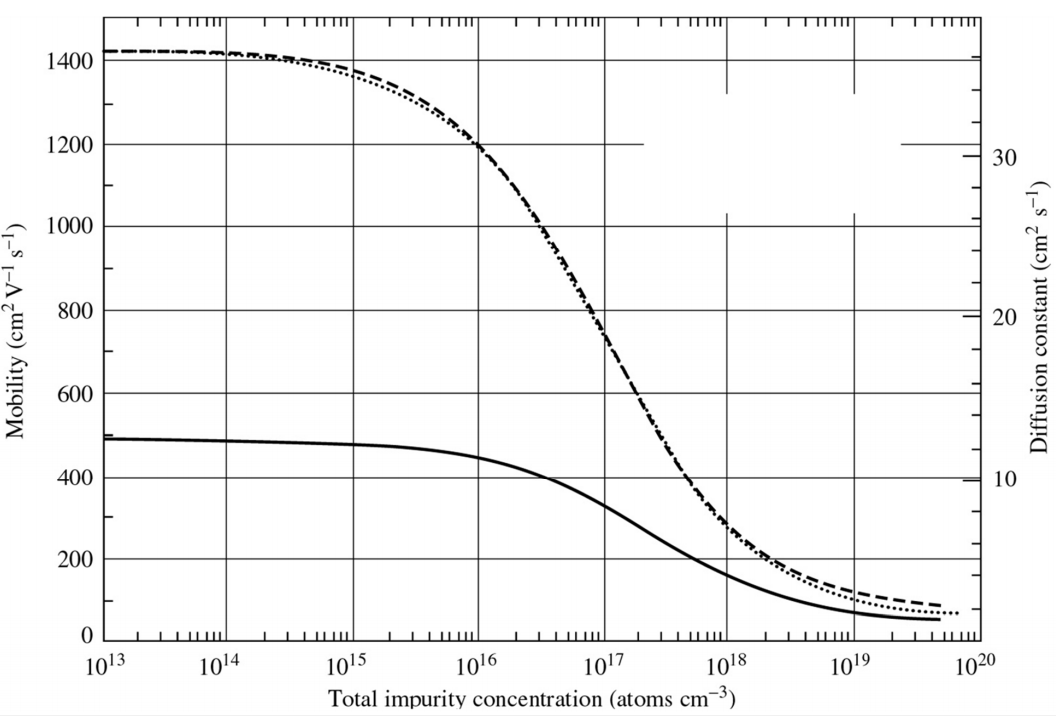
\includegraphics[width=1\linewidth]{DiffusionCoefficientChart.png}}
%\hspace{1em}
%\parbox[c]{4in}{\captionof{figure}{Diffusion Chart from Lecture I},
%\label{fig:pictureonright}}
%\end{minipage}

\begin{minipage}{\linewidth}
\centering
\raisebox{-.8in}{
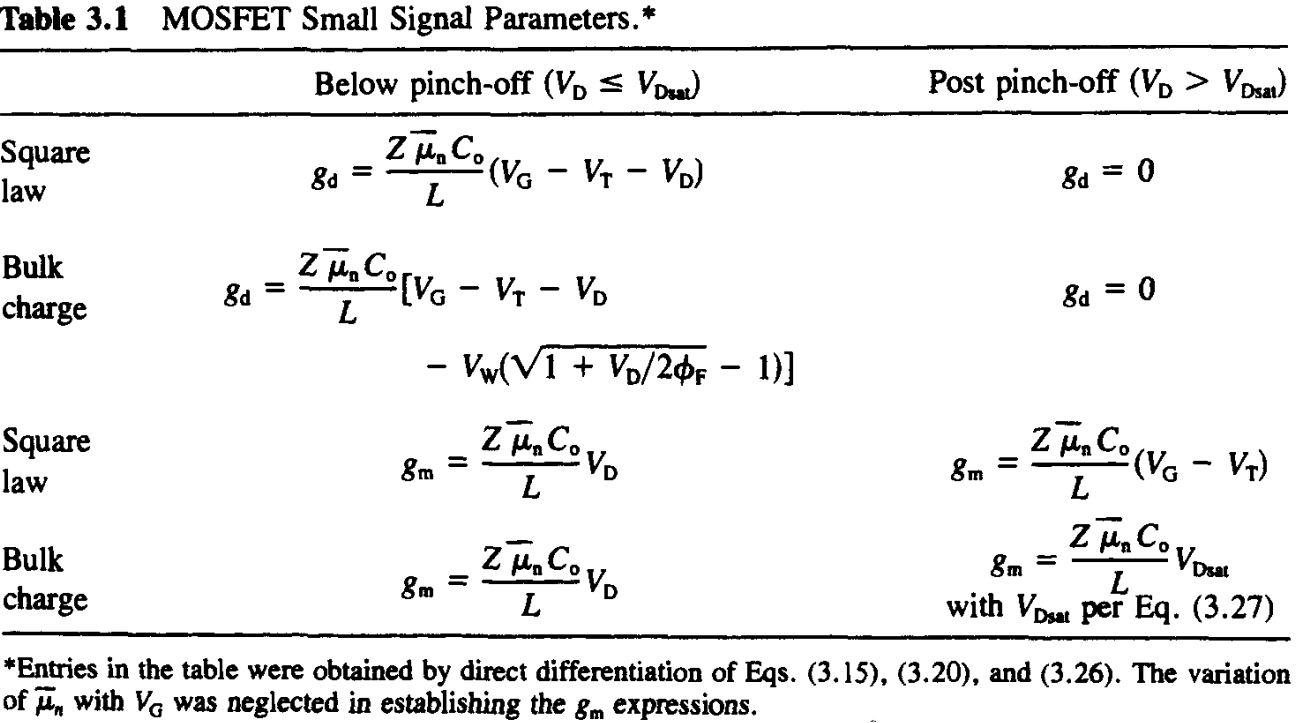
\includegraphics[width=1\linewidth]{MOSFETTable.png}}
\hspace{1em}
\parbox[c]{4in}{\captionof{figure}{Vol IV Mosfet table},
\label{fig:pictureonright}}
\end{minipage}
\begin{minipage}{\linewidth}
\centering
\raisebox{-.8in}{
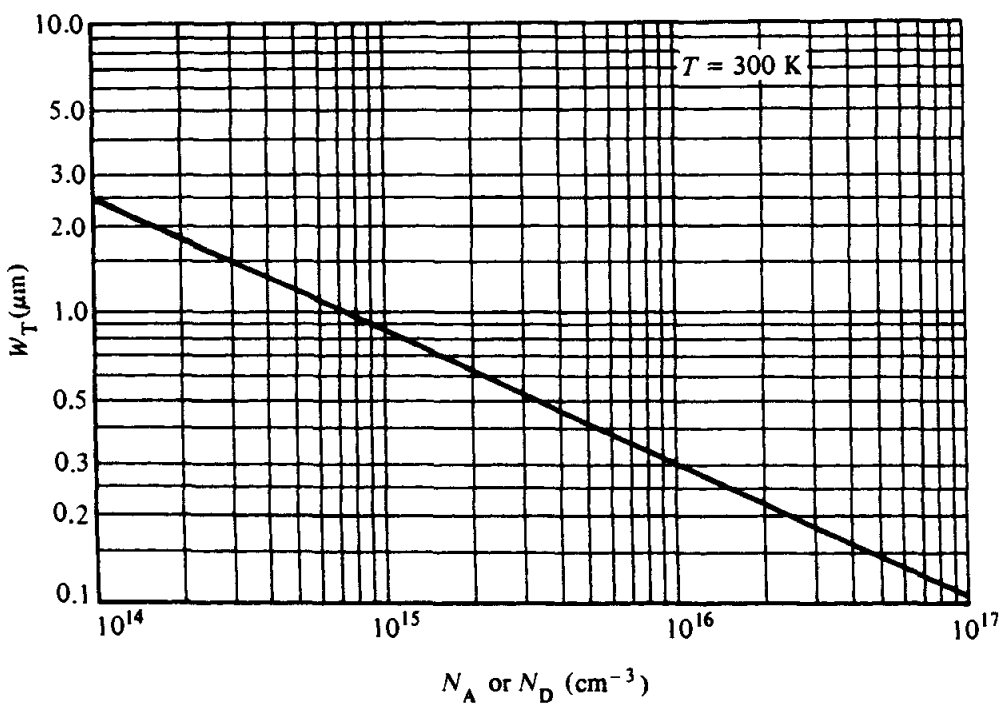
\includegraphics[width=1\linewidth]{MOSFETgraphdopants.PNG}}
\hspace{1em}
\parbox[c]{4in}{\captionof{figure}{Doping dependence of the maximum equilibrium depletion width inside silicon devices maintained at 300 K.},
\label{fig:pictureonright}}
\end{minipage}

\begin{minipage}{\linewidth}
	\centering
	\raisebox{-.8in}{
		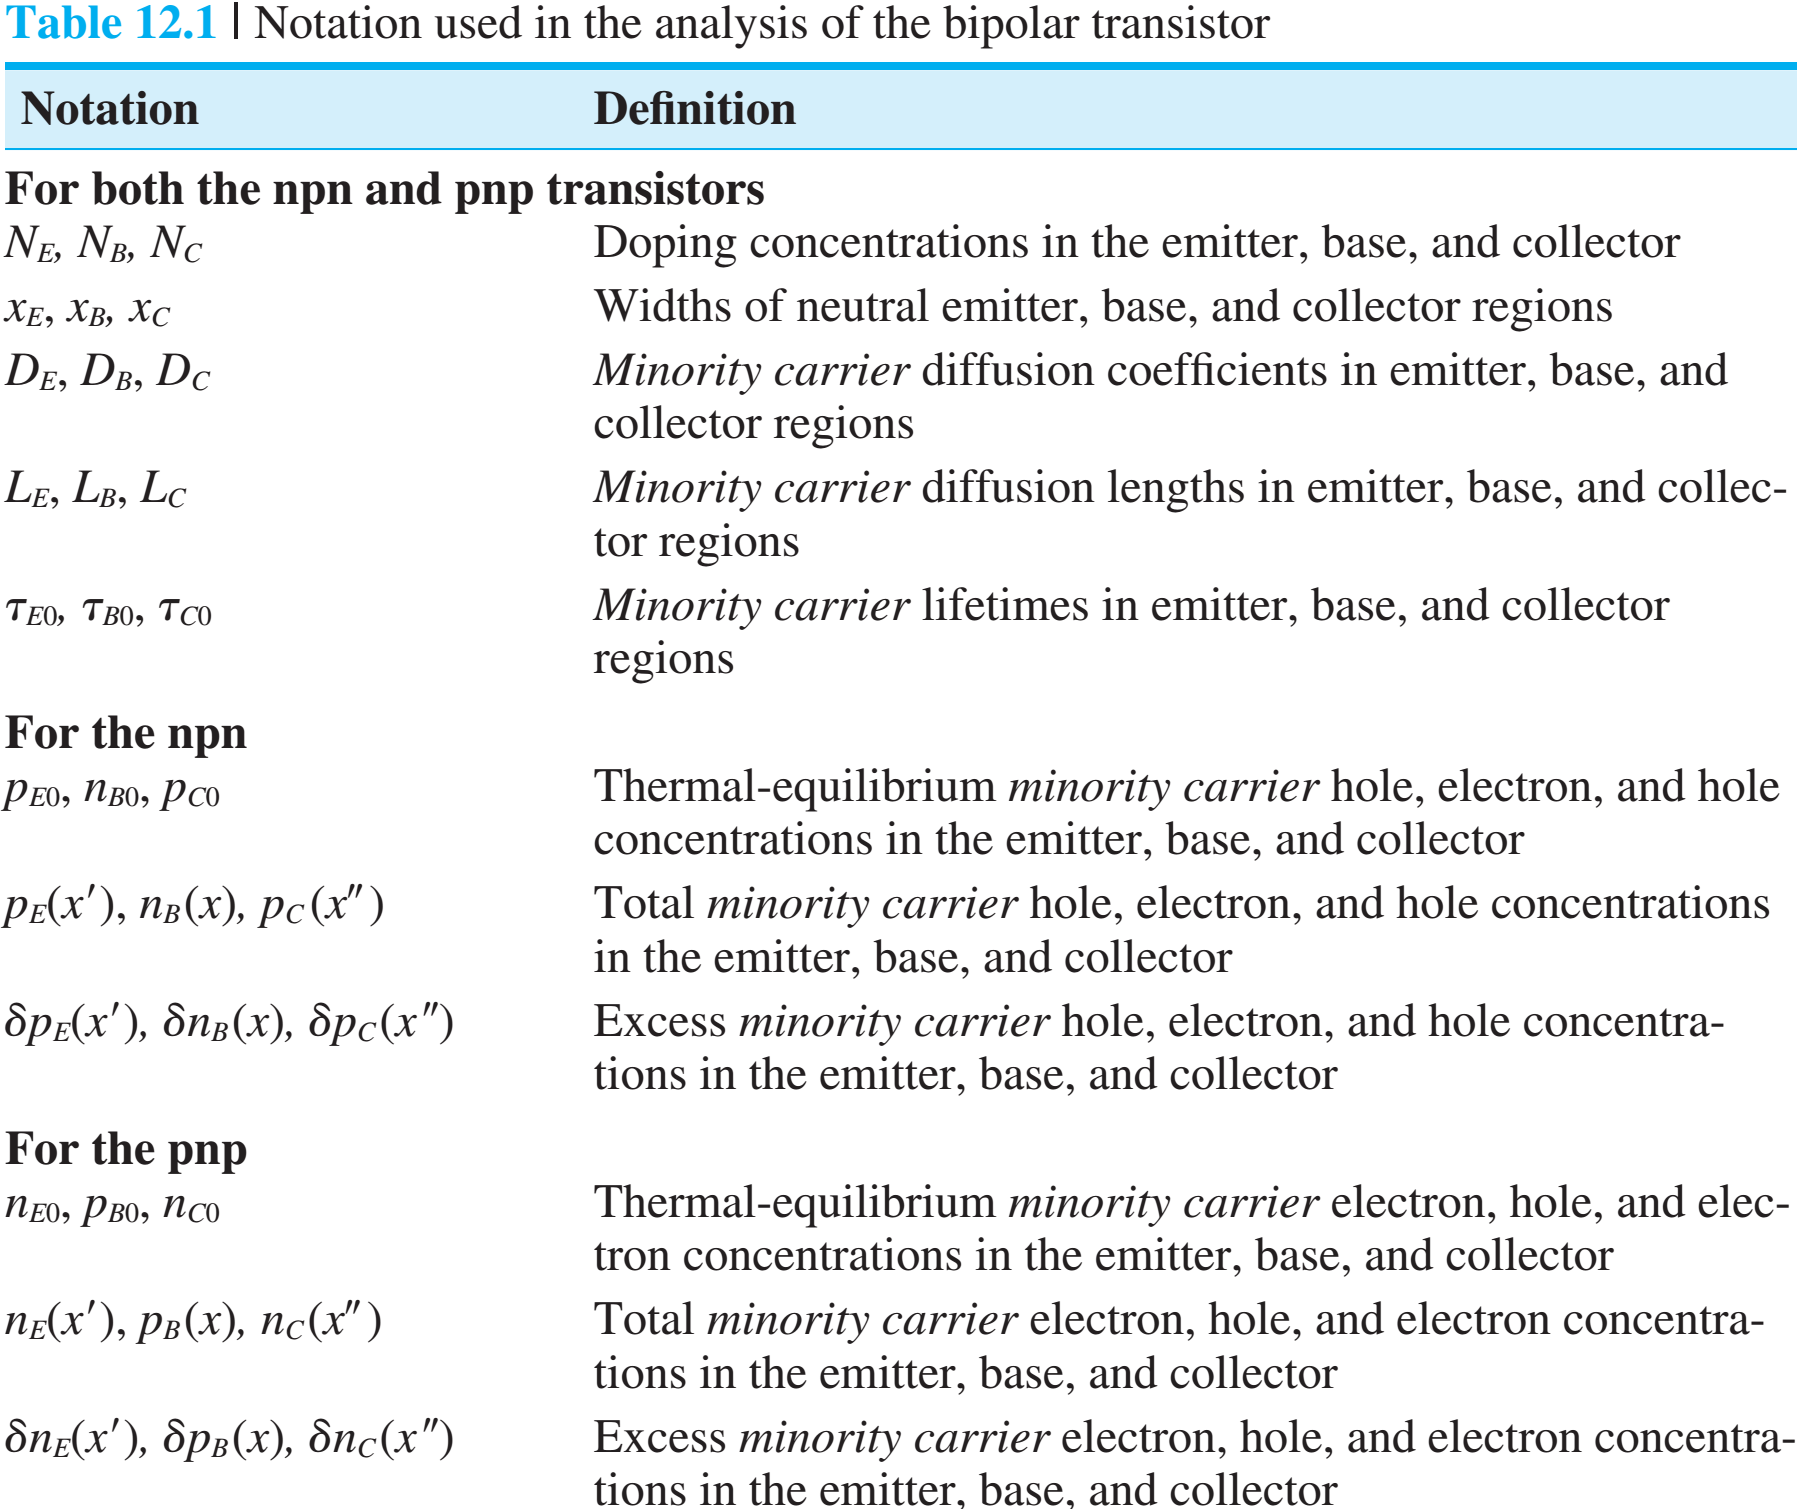
\includegraphics[width=1\linewidth]{NeamanTable12-1.png}}
	\hspace{1em}
	%\parbox[c]{4in}{\captionof{figure}{Resistivity Plot},
	\label{fig:pictureonrigh8194}
\end{minipage}
\begin{minipage}{\linewidth}
\centering
\raisebox{-.8in}{
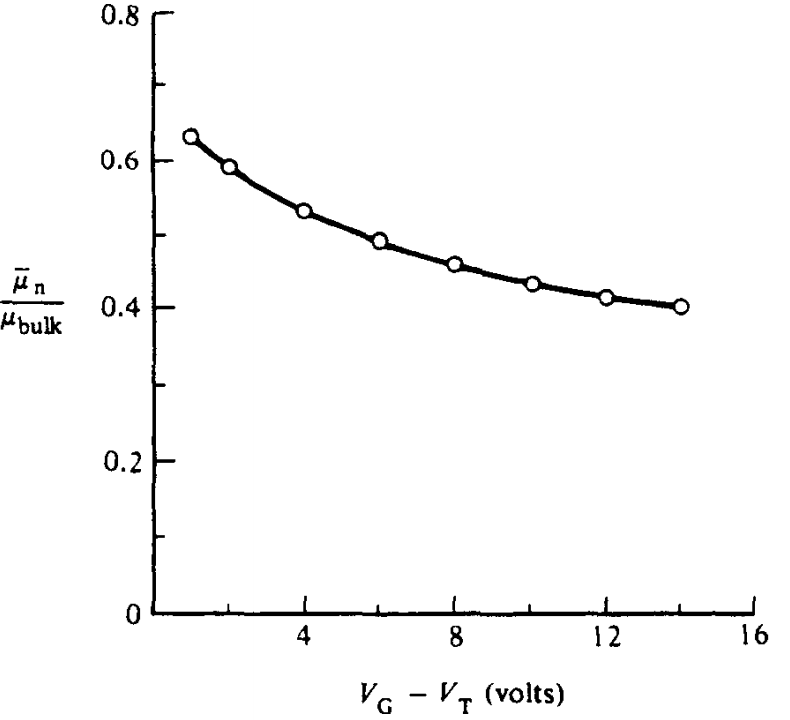
\includegraphics[width=0.6\linewidth]{MOSFETgraphVd_0.PNG}}
\hspace{1em}
\parbox[c]{4in}{\captionof{figure}{Vol IV Mosfet Gate voltages},
\label{fig:pictureonright}}
\end{minipage}

\begin{minipage}{\linewidth}
	\centering
	\raisebox{-.8in}{
		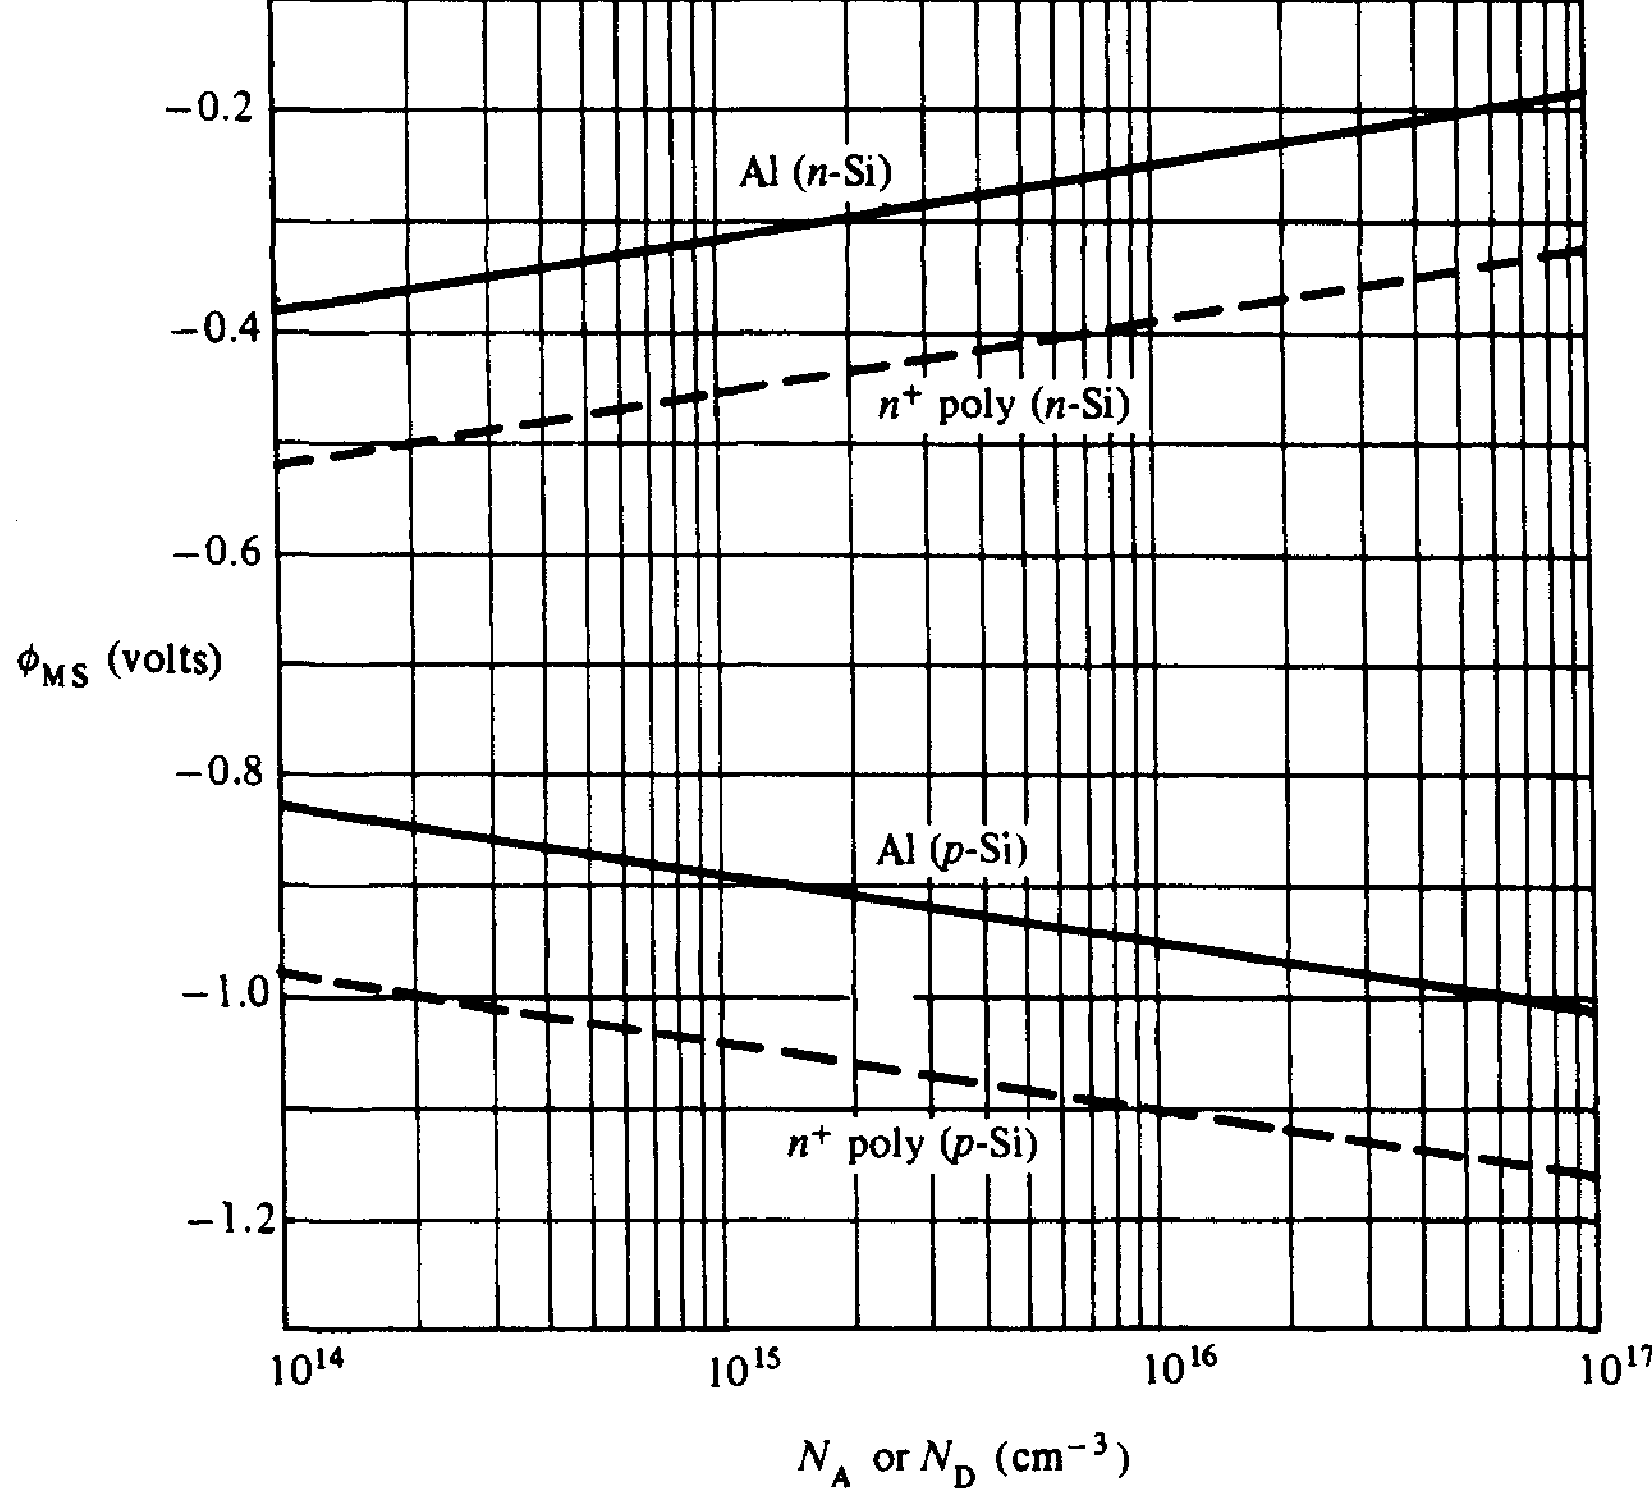
\includegraphics[width=1\linewidth]{Fig43VolIV.png}}
	\hspace{1em}
	\parbox[c]{4in}{\captionof{figure}{Workfunction difference as a function of a n- and p-type dopant conecntration in $n^+$ poly-Si-gate and Al-gate $SiO_2-Si$ structures. ($T=300 K$. $\phi_M^\prime-\chi^\prime=-0.18 \ eV$ for the $n^\prime$ poly-Si-gate structure; $\phi_M^\prime-\chi^\prime=0.03 eV$ for the Al-gate structure.)},
		\label{fig:pictureonright78}}
\end{minipage}
\begin{minipage}{\linewidth}
	\centering
	\raisebox{-.8in}{
		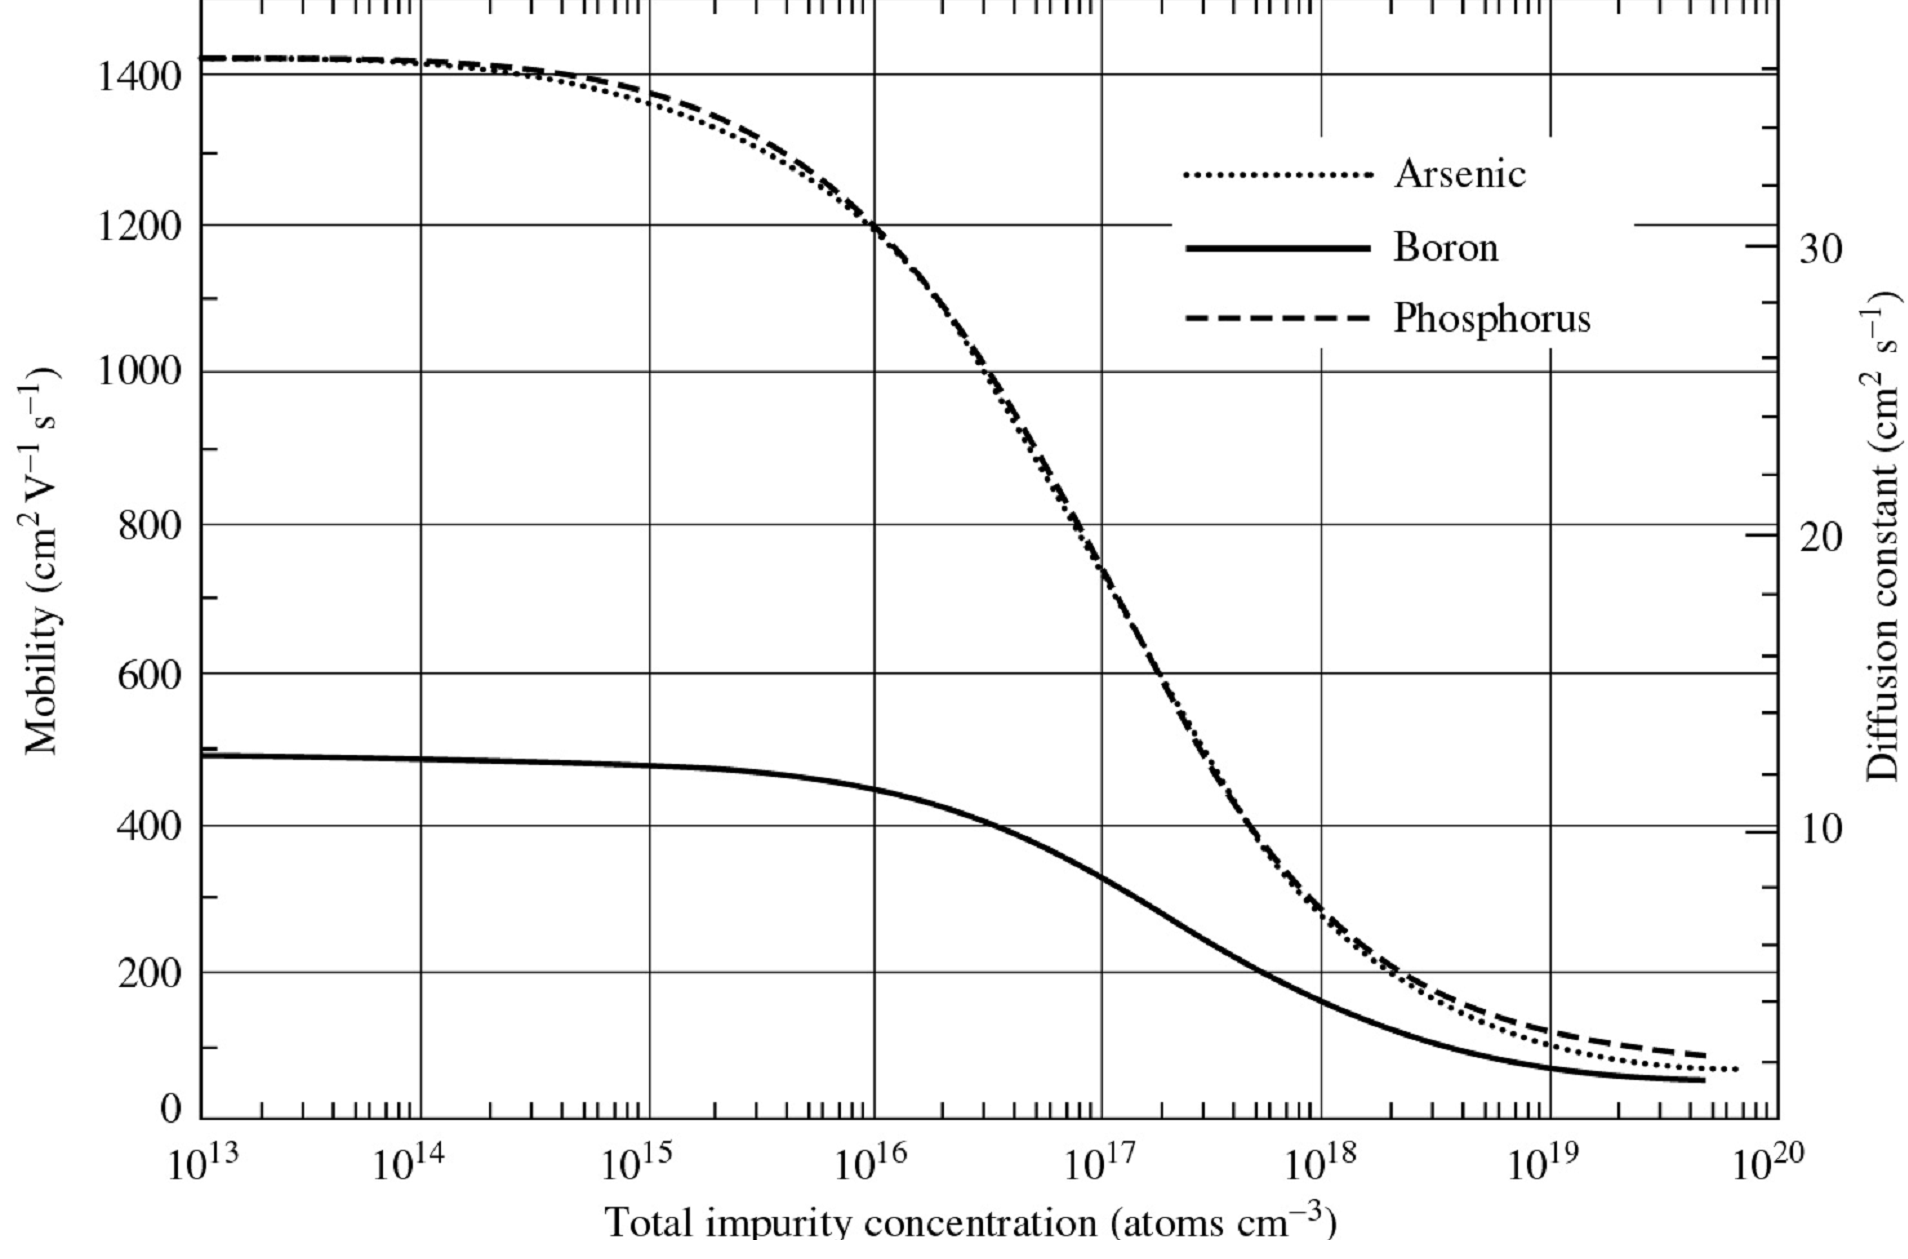
\includegraphics[width=0.7\linewidth]{GroupIIIGroupV.png}}
	%\hspace{1em}
%	\parbox[c]{4in}{\captionof{figure}{Boron Diffusion Chart},
		\label{fig:59}
\end{minipage}

\begin{minipage}{\linewidth}
	\centering
	\raisebox{-.8in}{
		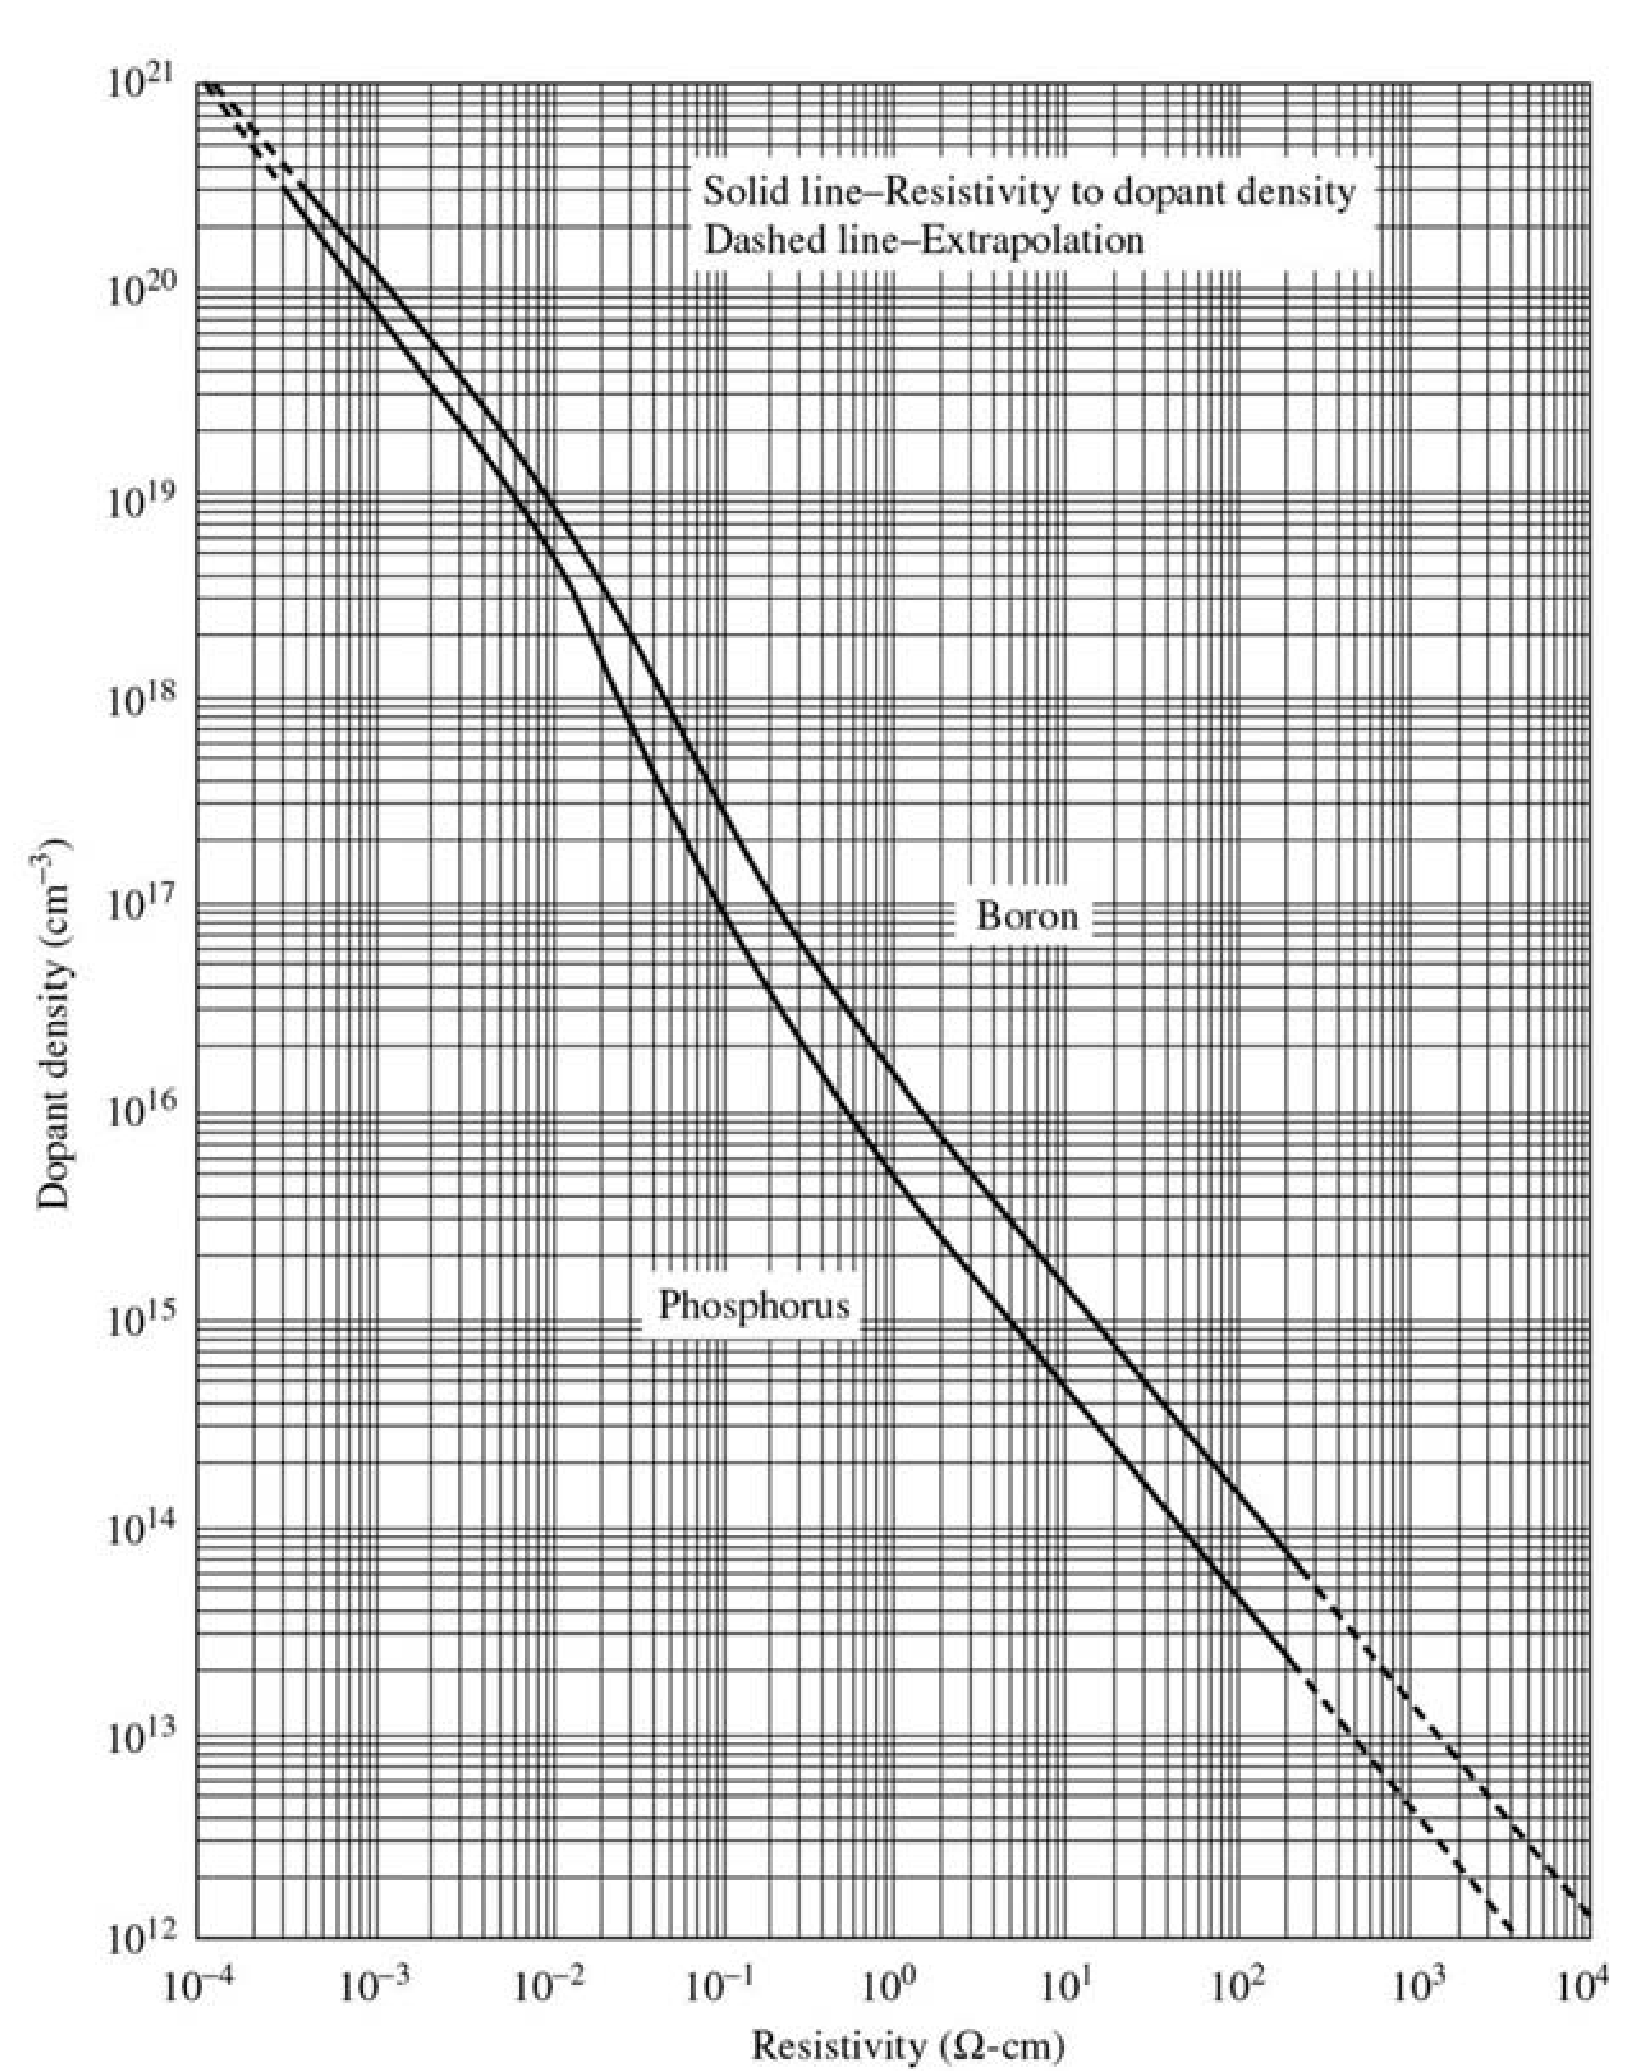
\includegraphics[width=0.7\linewidth]{boronChart.png}}
	\hspace{1em}
	\parbox[c]{4in}{\captionof{figure}{Boron Chart},
		\label{fig:4}}
\end{minipage}
\end{multicols}
\begin{minipage}{\linewidth}
	\centering
	\raisebox{-.8in}{
		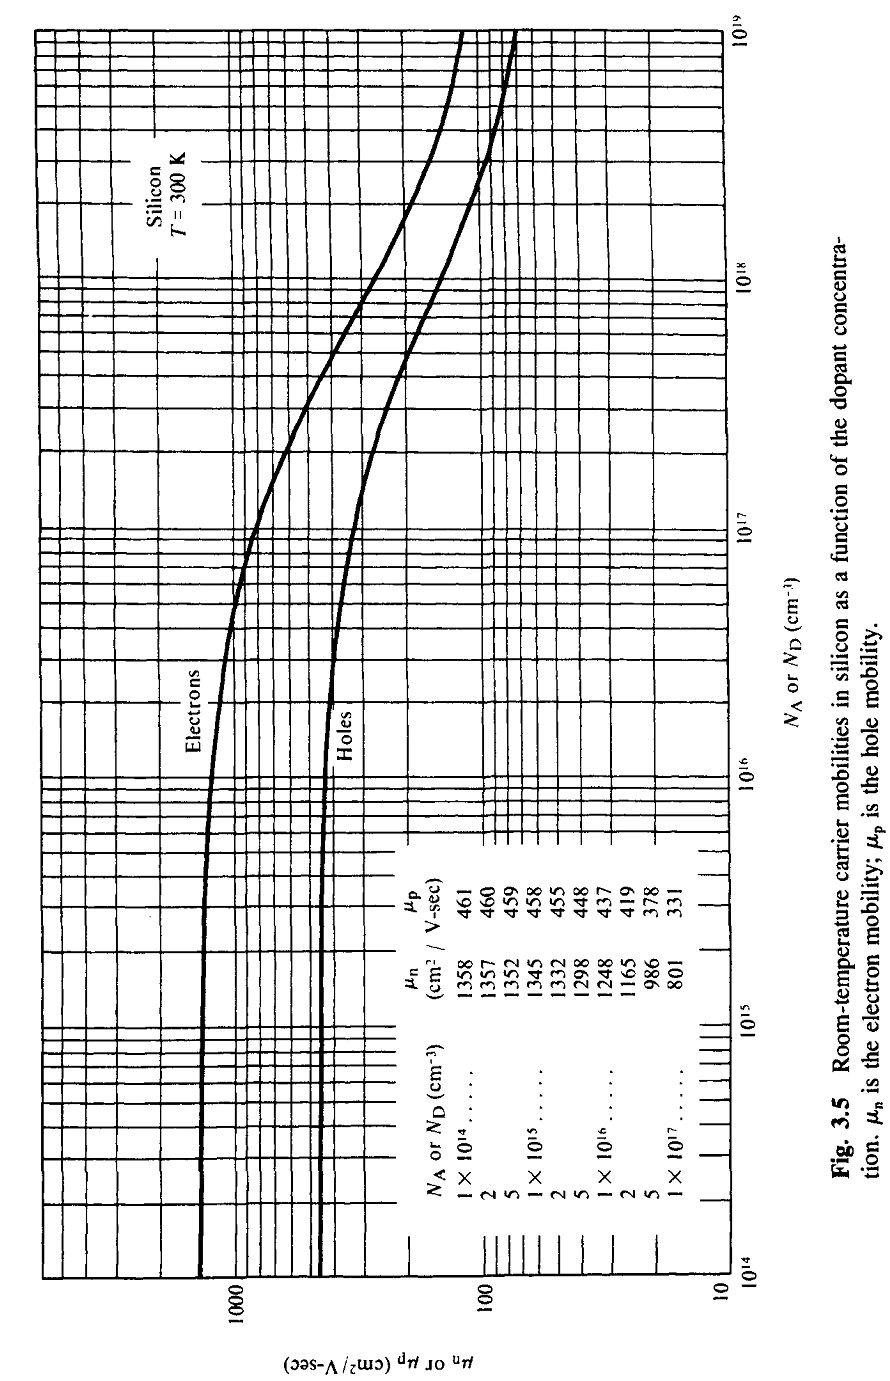
\includegraphics[height=1\textheight]{V1Figure3-5.png}}
% 	\hspace{1em}
% 	\parbox[c]{4in}{\captionof{figure}{Diffussion Constant},
% 		\label{fig:pictureonright79}}
\end{minipage}

\begin{minipage}{\linewidth}
	\centering
	\raisebox{-.8in}{
		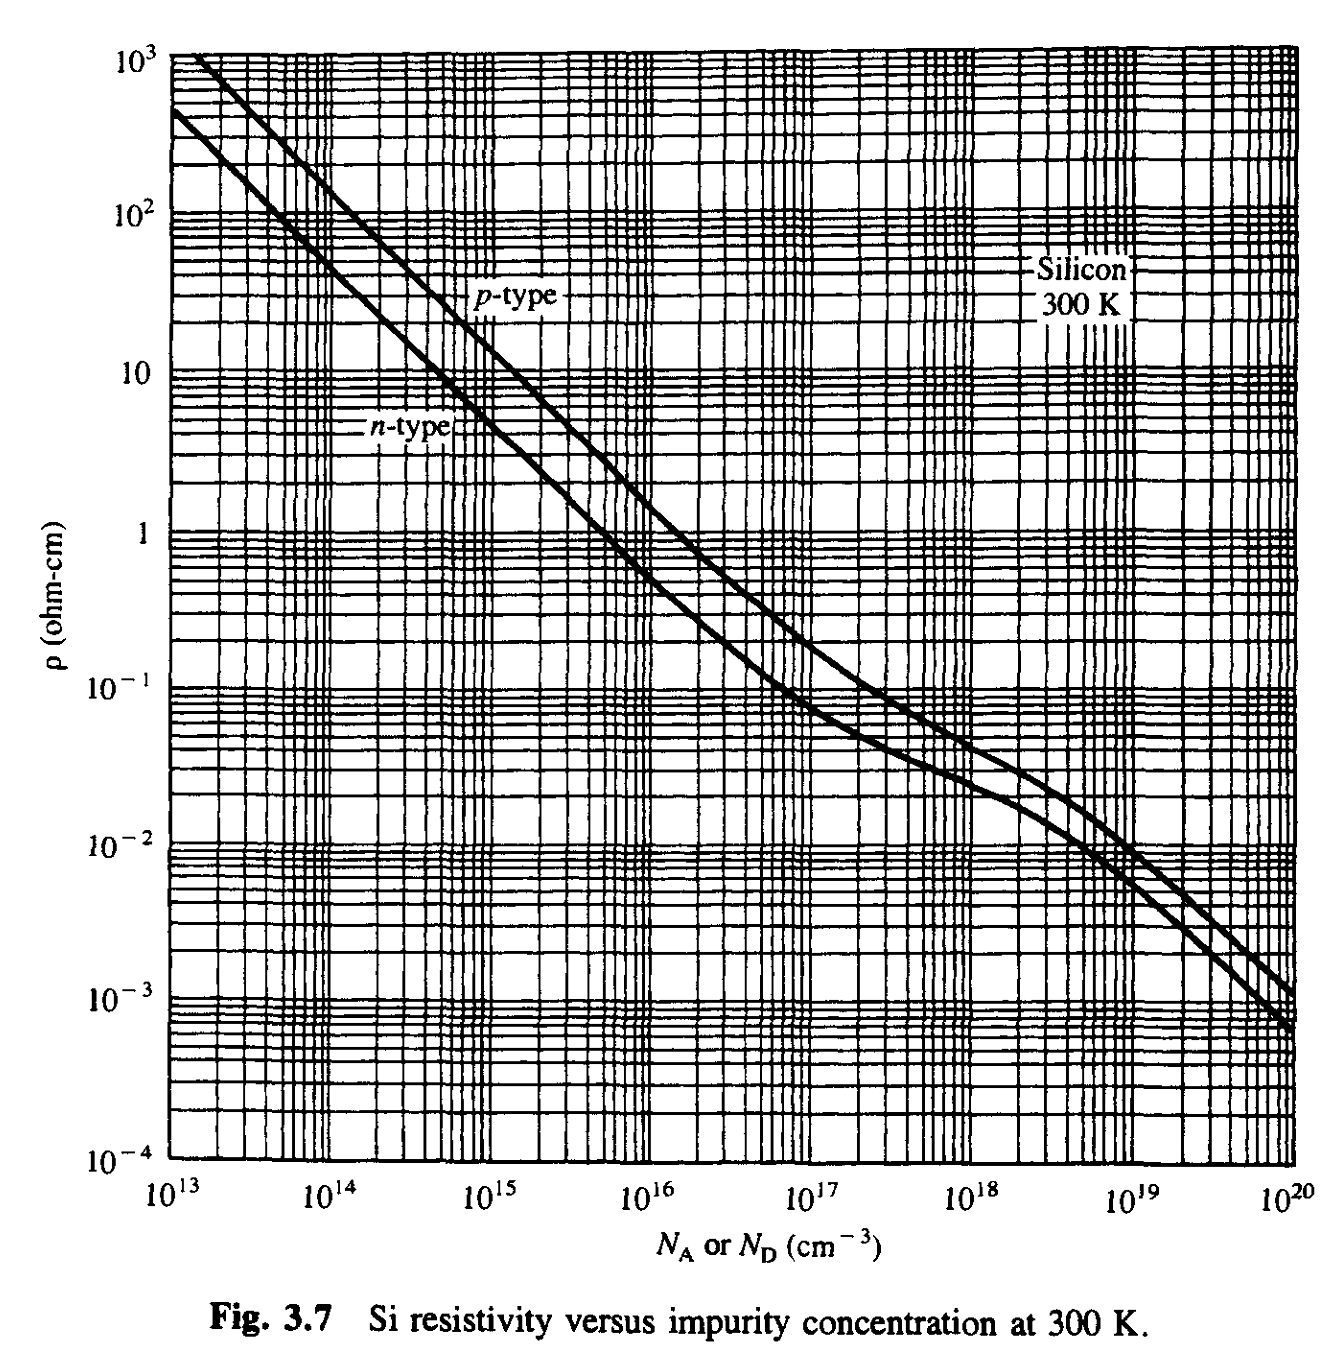
\includegraphics[width=1\textheight]{VIFigure3-7.png}}
	\hspace{1em}
	%\parbox[c]{4in}{\captionof{figure}{Resistivity Plot},
		\label{fig:pictureonrigh819}
\end{minipage}
% Exam material
\newpage 
\begin{forest}
	for tree={grow'=0}
[Important Topics
	[Section I
     [energy level quantization
     ]
     [Tunneling
     ]
     [SemiConductors
       [energy bands
       ]
       [doping levels
       ]
       [Fermi Levels
       ]
     ]
    ]
    [Section II
      [pn junctions
        [Ideal Diode Equation
        ]
        [metal Semiconductor 
         [Ohmic Contacts
         ]
         [Sckotty diodes
         ]
        ]
      ]
      [Band Edge Diagrams
      ]
    ]
    [Section III
      [Ebers-Moll Equation
      ]
      [Optimizating BJT Design
      ]
    ]
    [Section IV
      [Integrated Circuits
        [DRAM
        ]
        [floating gate
        ]
        [n-well design questions
        ]
      ]
      [MOSFET
        [threshold voltage
        ]
      ]
    ]
 ]
\end{forest}
I - 10 \%
II - 20 \%
III - 30 \%
IV  - 40 \%
\end{document}
